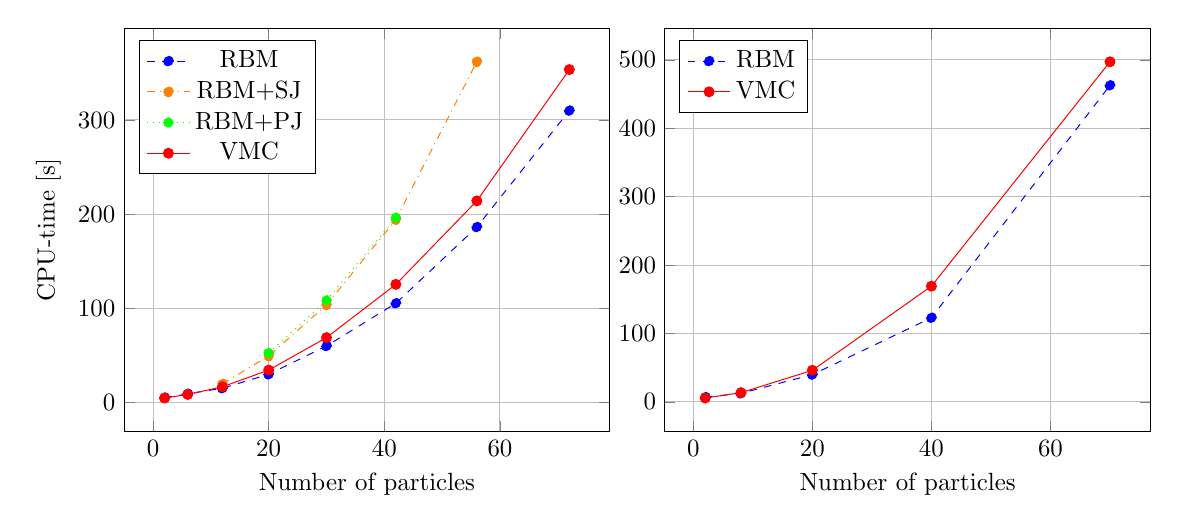
\begin{tikzpicture} [scale=0.9]
	\begin{axis}[name=2D, xlabel=Number of particles, ylabel={CPU-time [s]}, grid=major, legend pos=north west] 
	  \addplot[color=blue,mark=oplus*, dashed] coordinates { 
	  	 (2,5.141258)
	  	 (6,9.239086)
		 (12,15.17534) 
		 (20,29.92524) 
		 (30,60.01942) 
		 (42,105.3550) 
		 (56,186.3048)
		 (72,309.9558) }; 
	  \addlegendentry{RBM};
	  
	  \addplot[color=orange,mark=oplus*, dash dot] coordinates { 
	  	(12,19.79258) 
	  	(20,49.38614) 
	  	(30,103.70718) 
	  	(42,194.3012) 
	  	(56,361.7808) }; 
	  \addlegendentry{RBM+SJ};
	  
	  \addplot[color=green,mark=oplus*, dotted] coordinates { 
	  	(20,52.58098) 
	  	(30,108.3858) 
	  	(42,196.3522) }; 
	  \addlegendentry{RBM+PJ};
	  
	  \addplot[color=red,mark=oplus*] coordinates { 
	  	(2,4.7485)
	  	(6,8.551862)
	  	(12,16.69836) 
	  	(20,34.40414) 
	  	(30,68.92126) 
	  	(42,125.4514) 
	  	(56,214.0844)
	  	(72,353.5306) }; 
	  \addlegendentry{VMC};
	 \end{axis} 
	 \begin{axis}[name=3D, at=(2D.right of south east), anchor=left of south west, xlabel=Number of particles, grid=major, legend pos=north west] 
	 \addplot[color=blue,mark=oplus*, dashed] coordinates { 
	 	(2,6.717078)
	 	(8,12.33682)
	 	(20,39.74432) 
	 	(40,122.864) 
	 	(70,462.75) }; 
	 \addlegendentry{RBM};
	 
	 \addplot[color=red,mark=oplus*] coordinates { 
	 	(2,5.490018)
	 	(8,13.35986)
	 	(20,46.03914) 
	 	(40,169.0882) 
	 	(70,497.2244) };
	 \addlegendentry{VMC};
   \end{axis} 
\end{tikzpicture}